\newpage
\chapter{Badania}
%\textbf{Przerzucone z wcześniejszych rozdziałów:}
%\begin{itemize}
%\item W przypadku wszystkich opisanych w tym rozdziale algorytmów za \emph{warunkiem stopu} można rozumieć wykonanie z góry określonej maksymalnej liczby iteracji pętli lub brak poprawy najlepszego rozwiązania w pewnej liczbie ostatnich przebiegów algorytmu. 
%\item Do ustawiana elitismu w genetycznym i memetycznym - Tak również postąpiono w trakcie przeprowadzania badań w ramach tej pracy - wykorzystano domyślny w pakiecie \emph{GA} rozmiar grupy chronionych osobników wynoszący 5\% populacji.
%\end{itemize}


\section{Specyfikacja funkcji testowych}
Znajdowanie coraz lepszych metod rozwiązywania problemów optymalizacyjnych oraz ich testowanie jest zagadnieniem na tyle powszechnym, że powstały w tym celu narzędzia to ułatwiające. Dzięki ujednoliceniu sposobu badań wydajności algorytmów możliwe jest porównywanie ich na płaszczyźnie tych samych problemów. Jednym z pakietów języka \emph{R} powstałym w tym celu jest \emph{globalOptTests} \cite{globalOptTestsPackage}. Stanowi go zbiór kilkunastu funkcji o różnej liczbie parametrów. Każda z nich dodatkowo opisana jest dziedziną wartości poszczególnych argumentów oraz wartością funkcji w ekstremum. Wszystkie problemy zawarte w pakiecie są zadaniami znalezienia \emph{minimum} globalnego.
\par
Na potrzeby przeprowadzenia badań porównawczych różnych algorytmów wybrano z pakiety \emph{globalOptTests} 3 funkcje, które zostaną opisane poniżej. Reprezentują one problemy  optymalizacyjne o różnej wymiarowości. 
\subsection{Funkcja Schaffer nr 2}
%\begin{itemize}
%\item wzor
%\item wykres, bo 2D
%\item dziedzina argumentow
%\item optimum: 0, w początku układu współrzędnych
%\item cechy: wiele ekstremow lokalnych zblizonych do optimum, ale odseparowanych. Większość dziedziny rozwiązań jest płaska jak stół 
%\end{itemize}

\par
Funkcja \emph{Schaffer nr 2} jest przedstawicielem rodziny funkcji multimodalnych dwuwymiarowych zaproponowanych przez autora w ramach pracy doktorskiej związanej między innymi z problemami optymalizacyjnymi \cite{schaffer1985some}. Cechuje się ona posiadaniem wielu ekstremów lokalnych o podobnych wartościach do optimum. Przebieg funkcji zaprezentowany na rysunku \ref{fig:Schaffer1} i opisywana jest wzorem \ref{eq:Schaffer1}. Poszukiwanym ekstremum jest minimum osiągane w początku układu współrzędnych przestrzeni rozwiązań \ref{eq:Schaffer1_optim}. Przeszukiwana przestrzeń rozwiązań stanowi płaszczyznę $\Re^2$ ograniczoną do przedziału \ref{eq:Schaffer1_range}.
\begin{equation} \label{eq:Schaffer1}
f(x)=0.5+\frac{\sin^2(x_1^2-x_2^2)-0.5}{[1+0.001(x_1^2+x_2^2)]^2}
\end{equation}
\begin{equation} \label{eq:Schaffer1_optim}
f(x)=0 \Leftrightarrow x_1,x_2=0
\end{equation}
\begin{equation} \label{eq:Schaffer1_range}
x_1,x_2\in[-120,100]
\end{equation}
\par
Dokonując przeglądu funkcji dostępnych w ramach pakietu \emph{globalOptTests} natrafiono na nieścisłość nazewniczą. Opisywana w tym miejscu funkcja nazywana przez autora oraz w literaturze mianem \emph{Schaffer nr 2} (lub \emph{Schaffer N.2}) przez autora pakietu została nazwana funkcją \emph{Schaffer1}. Fakt, iż przynajmniej jedna z funkcji pakietu opatrzona jest inną nazwą niż powinna sprawia, że przed wykorzystaniem dowolnej innej funkcji z pakietu powinno się najpierw zweryfikować, czy jej implementacja jest zgodna z opisem w literaturze.

\begin{figure} 
\centering
\begin{subfigure}{.5\textwidth}
  \centering
  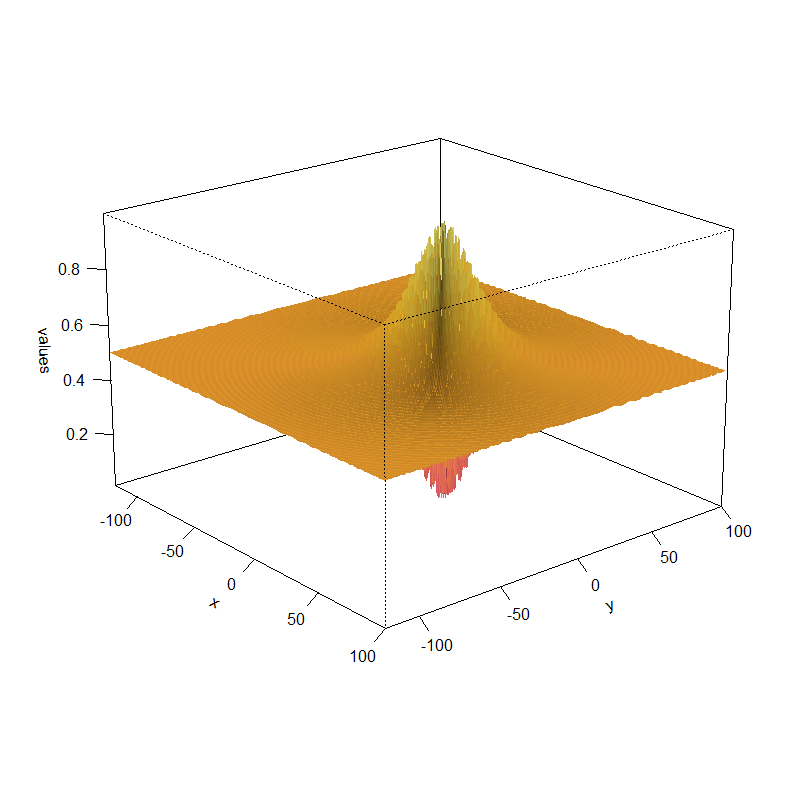
\includegraphics[width=\linewidth]{{img//roz03//Schaffer1_full_range.png}}
  \caption{ Pełna dziedzina argumentów}
  \label{fig:sub1}
\end{subfigure}%
\begin{subfigure}{.5\textwidth}
  \centering
  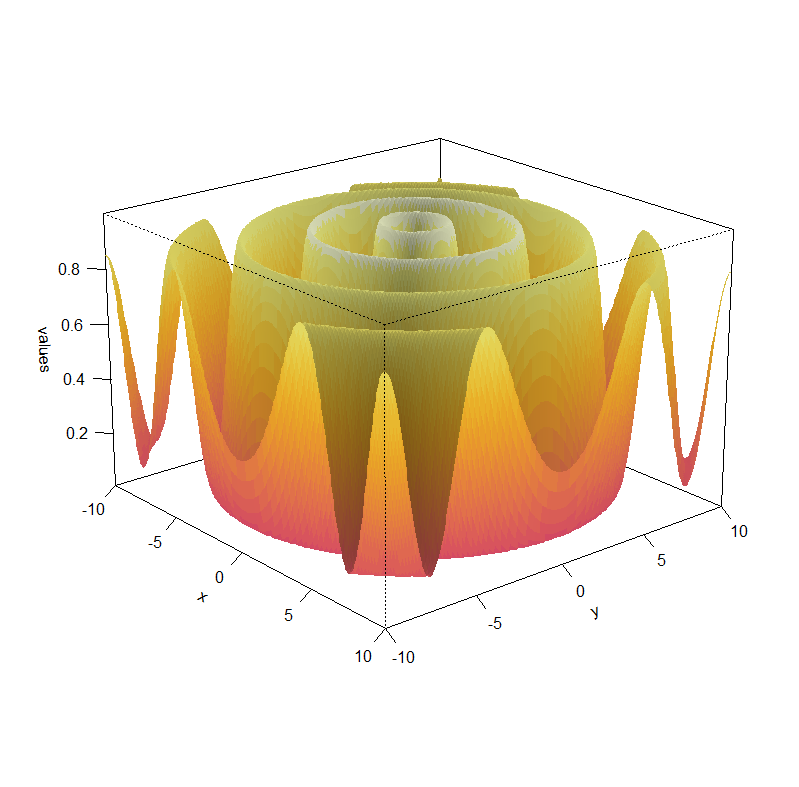
\includegraphics[width=\linewidth]{img//roz03//Schaffer1_small_range.png}
  \caption{Otoczenie optimum}
  \label{fig:sub2}
\end{subfigure}
\caption{Przebieg funkcji \emph{Schaffer nr 2}}
\label{fig:Schaffer1}
\end{figure}


\subsection{Funkcja Paviani}
%\begin{itemize}
%\item wzor
%\item dziedzina argumentow
%\item optimum: jakie i gdzie
%\item pewnie cos w necie ciekawego o nim jest
%\end{itemize}
\par
Drugą funkcją wykorzystaną w badaniach porównawczych jest funkcja \emph{Paviani}, która opisana jest wzorem \ref{eq:Paviani}. Została zaprezentowana w roli testowego problemu poddawanemu optymalizacji rzeczywistoliczbowej w ramach książki Davida Himmelblau'a \emph{Applied Nonlinear Programming} \cite{himmelblau1972applied}. Przestrzeń rozwiązań stanowi dziesięciowymiara przestrzeń ograniczona w przedziałach (\ref{eq:Paviani_range}). Podobnie jak \emph{Schaffer nr 2} jest ciągła i różniczkowalna w całej dziedzinie argumentów. Nietypowy zakres wartości parametrów jest konsekwencją zbieżności funkcji do nieskończoności dla wartości $x=2$ i $x=10$. Jedyne oszukiwane minimum funkcji osiągane jest dla wartości (\ref{eq:Paviani_optim}).
\begin{equation}\label{eq:Paviani}
f(x)=\sum_{i=1}^{10} \bigg(\log^2(x_i-2) + \log^2(10-x_i)\bigg) - \left(
\prod_{i=1}^{10} x_i\right)^{0.2}
\end{equation}
\begin{equation} \label{eq:Paviani_optim}
f(x)=-45.7784684040686 \Leftrightarrow x_i = 9.350266,\quad i = 1, ..., 10
\end{equation}
\begin{equation} \label{eq:Paviani_range}
x_i\in[2.0001,9.9999], \quad i=1,...,10
\end{equation}

\subsection{Funkcja ZeldaSine10}
Jako trzecią funkcję do testów badań wybrano \emph{ZeldaSine10}. Wybrano ją, ponieważ wstępne próby wykazały, że algorytmy znajdują dobre rozwiązania dopiero po większej liczbie iteracji niż miało to miejsce w przypadku omawianych powyżej funkcji \emph{Schaffera nr 2} i \emph{Paviani}. Funkcja opisana jest wzorem \ref{eq:ZeldaSine10}, a szukane minimum ma wartość $3.5$ (\ref{eq:ZeldaSine10_optim}). Podobnie do \emph{Paviani} jest multimodalna, ciągła, różniczkowalna i opierająca się na dziesięciowymiarowej dziedzinie parametrów, które mogą przyjmować wartości z przedziału~(\ref{eq:ZeldaSine10_range}). 
\begin{equation}\label{eq:ZeldaSine10}
f(x)=-2.5\prod_{i=1}^{10} \sin\left(x_i-\frac{\pi}{6}\right) - \prod_{i=1}^{10} \sin\left(5\left(x_i-\frac{\pi}{6}\right)\right)
\end{equation}
\begin{equation} \label{eq:ZeldaSine10_optim}
f(x)=-3.5 \Leftrightarrow x_i = \frac{2\pi}{3},\quad i = 1, ..., 10
\end{equation}
\begin{equation} \label{eq:ZeldaSine10_range}
x_i\in[0,\pi], \quad i=1,...,10
\end{equation}

\section{Platforma testowa}
%\begin{itemize}
%\item wersja R 3.3.3
%\item wersja GA 3.0.2
%\item wersja psoptim 1.0
%\item wersja rJava do komunikacji java-R 0.9-8
%\item wersja java 
%\item parametry techniczne komputera, co z parametrów może mieć wpływ na rezultaty oprócz: procesor i szybkość pamięci
%\item że pomimo możliwości uruchomienia zrównoleglonych wersji algorytmów nie zrobiono tego dla dokladniejszego ich porownania
%\item że testy przeprowadzono przy wykorzystaniu aplikacji powstałej na te potrzeby
%\item że aplikacja jest tylko nakładką na R i nie ma żadnego wpływu na szybkość i skuteczność działania testowanych algorytmów
%\item że dokładny opis aplikacji znajduje się w dodatku \ref{ch:dodatekA-aplikacja}
%\end{itemize}
\par
Niniejsza praca magisterska ma na celu porównanie efektywności, a przez to użyteczności w praktycznym zastosowaniu, algorytmu memetycznego względem innych metod optymalizacji. Do przeprowadzenia badań wykorzystano skrypty języka R zawarte w dodatku \ref{ch:dodatekB-wykorzystane skrypty}. Aplikacja powstała w trakcie pracy, a dokładniej opisana w dodatku \ref{ch:dodatekA-aplikacja} stanowi narzędzie umożliwiające wykorzystanie części z wspomnianych skryptów do optymalizacji problemów definiowanych przez użytkownika.
\par
Na specyfikację platformy testowej składają się dwa aspekty: parametry techniczne komputera oraz wersje wykorzystanych narzędzi. Szczególnie drugi aspekt może mieć znaczenie w przypadku próby porównania otrzymanych rezultatów z wynikami badań przedstawionymi w literaturze. Różne wersje narzędzi mogą w odmienny sposób implementować ten sam mechanizm optymalizując działanie algorytmów lub poprawiając wydajność interpretera skryptów. Należy również zaznaczyć, że pakiet \emph{GA} umożliwia wykonanie analizowanych algorytmów w wersji zrównoleglonej, jednakże dla spójności porównania z PSO nie skorzystano z tej opcji.
\begin{table}[hb]
\label{table:wykorzystane_narzedzia}
\caption{Wersje i funkcje wykorzystanych narzędzi}
\begin{tabularx}{\textwidth}{|l|c|X|}
	\hline
	Narzędzie & Wersja & Funkcja \\
	\hline
	R & 3.3.3 & Interpreter języka \\
	Pakiet \emph{GA} & 3.0.2 & Zawiera implementacje m. in. algorytmu genetycznego i memetycznego \\
	Pakiet \emph{psoptim} & 1.0 & Zawiera implementację algorytmu PSO \\
	Pakiet \emph{rJava} & 0.9-8 & Interfejs komunikacyjny z językiem Java (wykorzystany w aplikacji) \\
	JRE & 1.8.0\_111 & Środowisko uruchomieniowe aplikacji \\
	\hline
	\end{tabularx}
\end{table}
\par
Podzespołami komputera mogącymi wpłynąć na uzyskiwane czasy wykonania algorytmów w głównej mierze są procesor i pamięć RAM. W przypadku rezygnacji z zrównoleglonej wersji algorytmów największe znaczenia ma wydajność pojedynczego rdzeni procesora. W przypadku pamięci RAM istotna jest nie jej pojemność, a szybkość dostępu, jednakże jej wpływ jest drugorzędny. Dokładna specyfikacja wykorzystanych podzespołów przedstawia tabela \ref{table:parametry_komputera}.
\begin{table}[hb]
\caption{Parametry sprzętowe maszyny testowej}
\label{table:parametry_komputera}
\begin{center}
\begin{tabular}{|l|l|}
	\hline
	Podzespół & Opis \\
	\hline
	Procesor & Intel i7-3610QC 2.3GHz \\
	Pamięć RAM & Kingstone DDR3 800MHz 11CL \\
	\hline
	\end{tabular}
\end{center}
\end{table}



\section{Przyjęte miary efektywności algorytmów}
\label{sec:przyjete_miary_efektywnosci_algorytmow}
%wszystko dla tych samych liczby iteracji
%\begin{enumerate}
%\item najlepsze znalezione rozwiązanie kolejno w iteracjach
%\item średnie rozwiązanie populacji kolejno w iteracjach
%\item czas osiągnięcia rozwiązań 90, 95 i 99\% danej konfiguracji, a nie globalnego optimum
%\item \% skuteczności, czyli ile procent wywołań znajduje rozwiązanie w ogległości 0.005*range.
%\end{enumerate}

\par
W tym podrozdziale zostaną omówione miary przyjęte w trakcie porównywania różnych algorytmów ze sobą. Kryterium decydującym w trakcie doboru parametrów algorytmów opisanego w rozdziale \ref{ch:przyjety_model_doboru_parametrow_algorytmu} była pierwsza z poniżej opisanych ocen - \emph{kryterium nr 1}. Aspekty algorytmów brane pod uwagę w porównaniach są odpowiednio zaadaptowanymi kryteriami porównawczymi z innych prac badawczych powstałych wokół tego tematu. Starano dobrać się je w taki sposób, by jak najlepiej opisywały zarówno jakość znajdowanego rozwiązania (\emph{kryterium nr 1}) jak i szybkość dochodzenia do satysfakcjonującego rezultatu (\emph{kryterium nr 2}). Osobnym aspektem branym pod uwagę jest również powtarzalność skutecznego działania algorytmu (\emph{kryterium nr 3}) oraz to, jak wykorzystanie poszczególnych algorytmów wpływa na różnorodność i charakterystykę całej populacji (\emph{kryterium nr 4}).

\par 
Najprostszym i zarazem najbardziej intuicyjnym sposobem zdefiniowania efektywności algorytmu jest jakość znajdowanego rozwiązania. Za jakość rozumiana jest tutaj bliskość względem poszukiwanego minimum w kontekście wartości funkcji celu, a nie odległości znalezionego wektora parametrów od rozwiązania optymalnego w wielowymiarowej przestrzeni rozwiązań. \emph{Kryterium nr 1} może być uważane za najważniejsze w przypadku zamiaru wykorzystania algorytmu w sytuacji, w której priorytetem jest dokładność znalezionego rozwiązania, a nie czas potrzebny na jej znalezienie. 
\par
Badania prowadzone pod kątem \emph{kryterium nr 1} będą polegać na wykonywaniu się pętli algorytmów aż do momentu uzyskania zbieżności rozwiązań. Przyjętym symptomem takiej sytuacji jest brak poprawy znajdowanego rezultatu w ciągu ostatnich 10 iteracjach. Rezultaty zostaną porównane zarówno pod kątem najlepszych uzyskanych rozwiązań w populacji, ale i liczby iteracji potrzebnych do ich uzyskania. Analogiczne kryterium porównawcze efektywności algorytmów wykorzystano w pozycjach literaturowych \cite{boyabatli2004parameter}, \cite{elbeltagi2005comparison} i \cite{ong2006classification}
%(najlpesze znalezione rozwiazacanie, wstepnie $l_iter=25$ skoro dla 5 wyniki już były całkiem całkiem)

\par
%(czas osiagniecia 90, 95, 99% dokladnosci rozwiazan, dla przynajmniej takiej liczby iteracji pozwalającej na uzyskanie sukcesu)
Drugą przyjętą miarą efektywności algorytmów - \emph{kryterium nr 2} - jest czas potrzebny na osiągnięcie rozwiązania o określonej dokładności. Porównanie oparte zostanie na pięciu progowych wartościach dokładności rozwiązań: 50\%, 75\%, 90\%, 95\% i 99\%. Dokładność rezultatu określana jest na podstawie wzoru \ref{eq:kryterium_2_dokladnosc}. 
\par
Oczywistym jest, że dodatnie dodatkowych mechanizmów do prostego schematu realizowanego przez algorytm genetyczny opisany w rozdziale \ref{ch:charakterystyka_algorytmow_ewolucyjnych} spowoduje ograniczenie szybkości przetwarzania kolejnych pokoleń symulacji ewolucji. Przedstawienie wyników badań w dziedzinie rzeczywistego czasu wykonania algorytmu pozwoli określić, czy wolniejsze wykonanie algorytmu skutkować będzie lepszą jakością rozwiązań w populacji. W tym miejscu należy również pamiętać o specyfice przyjętego modelu algorytmu memetycznego, a mianowicie o przeprowadzaniu dodatkowego doskonalenia najlepszego osobnika po spełnieniu warunku stopu. Wstępne próby wykazały, że to ostanie przeszukanie lokalne może w znacznym stopniu poprawić jakość rozwiązania. Monitorując rezultaty w trakcie działania algorytmu nie będzie możliwości uwzględnienia tej ostatniej optymalizacji osobnika. Fakt ten może ujawniać się w uzyskanych rezultatach badań tym, że jakość rozwiązań obserwowanych w czasie działania algorytmu będzie znacznie gorsza, od tych uzyskanych dla \emph{kryterium nr 1} przy porównywalnej liczbie iteracji. Podobną miarę efektywności przyjęto w publikacjach \cite{elbeltagi2005comparison} i \cite{mullen2014continuous}.
\begin{equation} \label{eq:kryterium_2_dokladnosc}
dokładność = \left(1-\frac{r_{best}-r_{opt}}{r_{ref}-r_{opt}}\right)*100\%
\end{equation}
gdzie:
\[r_{opt} - szukane\; minimum\; funkcji\; przystosowania\]
\[r_{best} - średnie\; najlepsze\; rozwiązanie\; populacji\; w\; danej\; chwili\]
\[r_{ref} - rozwiązanie\; odniesienia - średnie\; rozwiązanie\; losowo\; wygenerowanej\; populacji\]


\par 
%\cite{mullen2014continuous} \cite{elbeltagi2005comparison}
Kolejną przyjętą miarą efektywności algorytmów - \emph{kryterium nr 3} - stanowi powtarzalność osiągania satysfakcjonującego rozwiązania, za które przyjęto takie spełniające warunek opisany wzorem \ref{eq:kryterium_3_warunek}. W odróżnieniu od pozostały pozostałych kryteriów analizowana jest tutaj nie uzyskana wartość funkcji dopasowania znalezionego rozwiązania, a jego położenie w przestrzeni rozwiązań poprzez odległość euklidesowa od rozwiązania optymalnego.
\par 
W przypadku tego kryterium porównywane algorytmy uruchamiane zostaną z taką samą maksymalną liczbą iteracji będącą warunkiem stopu. O ile w pozostałych kryteriach wszystkie rezultaty są wartościami uśrednionymi z pełnej puli wywołań optymalizacji, o tyle w tym przypadku rozpatrywane i zliczane zostaną kolejne wywołania z osobna. Wykorzystana w tym miejscu maksymalna liczba iteracji zostanie określona na etapie doboru parametrów algorytmów zgodnie z scenariuszami przedstawionymi w rozdziale \ref{sec:badane_scenariusze_doboru_parametrow} dla każdej z wykorzystanych funkcji testowych z osobna. W przypadku, gdy preferowane przez algorytmy liczby iteracji będą różne wybrana zostanie wartość najmniejsza z nich. Ta miara efektywności zaczerpnięta została z publikacji \cite{elbeltagi2005comparison} i \cite{mullen2014continuous}. 
\begin{equation} \label{eq:kryterium_3_warunek}
\sum_{i=1}^{n}\left(opt_i-r_i\right)^2 < x*\sum_{i=1}^{n}\left(max_i-min_i\right)^2
\end{equation}
gdzie:
\[opt - wektor\; atrybutów\; szukanego\; rozwiązania\; optymalnego\]
\[r - wektor\; atrybutów\; najlepszego\; znalezionego\; rozwiązania\]
\[min - wektor\; dolnych\; ograniczeń\; dziedziny\; rozwiązań\]
\[max - wektor\; górnych\; ograniczeń\; dziedziny\; rozwiązań\]
\[x \in \lbrace0.005, 0.01, 0.015\rbrace\]
%(\% skuteczności dla tej samej liczby iteracji, wstepnie $l_iter=25$)

\par 
%(średnie rozwiazanie populacji dla tej samej liczby iteracji, wstepnie $l_iter=25$)
Ostatnim przyjętym kryterium porównawczym - \emph{kryterium nr 4} - jest ogólna różnorodność genetyczna populacji określana poprzez różnicę wartości średniego przystosowania wszystkich osobników i najlepszego z nich. Im mniejsza ta różnica tym większa zbieżność kodowanych rozwiązań, a więc koncentracja wokół najlepszego osobnika. Taka sytuacja może mieć negatywne skutki w przypadku zdominowania populacji przez jednostki skoncentrowane w pobliżu jednego z lokalnych ekstremów co zmniejsza zdolności poznawcze ogółu populacji, zmniejsza jej różnorodność genetyczną co może zmniejszyć szansę znalezienia rozwiązania optymalnego. To kryterium zostało oparte o analogiczne przedstawione w publikacji \cite{ong2006classification}. W przypadku tego kryterium analizowana będzie zmienność opisanej wyżej różnorodności populacji na przestrzeni 100 pokoleń.



